\documentclass[12pt]{article}

%%%%%%%%%%%%%%%%%%%%%%%%%%%%%%%%%%%%%%%%%%%%%%%%%%%%
% Preamble:
%%%%%%%%%%%%%%%%%%%%%%%%%%%%%%%%%%%%%%%%%%%%%%%%%%%%
% Typical Packages:
\usepackage[utf8]{inputenc}
\usepackage{fullpage}
\usepackage{amsfonts}
\usepackage{amsmath}
\usepackage{amsthm}
\usepackage{amssymb}
\usepackage{mathrsfs}
\usepackage{graphicx}
\usepackage{color}
\usepackage{palatino}
\usepackage{url}
\usepackage{multicol}
\usepackage{enumerate}
\usepackage{ulem}
\usepackage{tikz}
\usepackage{tipa}
\usepackage{upgreek}
\usepackage{hyperref}
\usepackage{verbatim}
\usepackage{caption}
\usepackage{fancyhdr}

\thispagestyle{empty}

% Fancy Header Package:
\usepackage{fancyhdr}
\setlength{\headheight}{15.2pt}
\pagestyle{fancy}
\setlength\headsep{30pt}
\lhead{Mini-Project 4 Report}
\rhead{Trevor Wylezik}

%%%%%%%%%%%%%%%%%%%%%%%%%%%%%%%%%%%%%%%%%%%%%%%%%%%%
% Title:
%%%%%%%%%%%%%%%%%%%%%%%%%%%%%%%%%%%%%%%%%%%%%%%%%%%%
\title{Mini Project 4 - Data Analytics}
\author{Trevor Wylezik}
\date{\today}



%%%%%%%%%%%%%%%%%%%%%%%%%%%%%%%%%%%%%%%%%%%%%%%%%%%%
% Start Document:
%%%%%%%%%%%%%%%%%%%%%%%%%%%%%%%%%%%%%%%%%%%%%%%%%%%%
\begin{document}

\maketitle

\abstract
{\noindent
In a world that is becoming more and more technical, data is one of the most important aspects of a company or government. However, collecting all of this data has to be put somewhere and eventually sifted through. Data analytics is the process of using tools and technologies to collect insight from data to solve problems. For example, the insurance industry has specific teams of actuaries to perform data analytics on the insurance claims incurred to summarize the data, clear the noise, and update their prices accordingly. In this project, we will investigate two large datasets from iMDb and Rotten Tomatoes on movies. These datasets will include key information like the title of the movie, genre, rating certificate, critics/audience scores, and much more. Using tools like excel and python, we can find trends in the data to understand the movies industry at a higher level. Graphs and charts will be produced to have a convenient way to understand these trends.
}

\newpage


%%%%%%%%%%%%%%%%%%%%%%%%%%%%%%%%%%%%%%%%%
% Introduction Section: 
%%%%%%%%%%%%%%%%%%%%%%%%%%%%%%%%%%%%%%%%%
\section{Introduction}
In this report, we will investigate two large datasets from iMDb and Rotten Tomatoes. These are movie review companies that keep track of the movies they review and their critics scores as well as the audience scores for the movies. First, we will explore the datasets in excel to understand the big picture. Then, the data will be cleaned in python to produce a more convenient dataset to work with. This will be done for both datasets. Finally, certain topics can be investigated and charts can be produced to help investigate the differences between the two companies and trends within their own data. \\

\noindent This project is organized as follows: in Section 2, we will highlight the problem statement. In section 3, we will introduce the datasets and go deeper in to the cleaning of the dataset. Section 4 and 5 will be the final results and charts of the project and a discussion about the results. \\

\section{Problem Statement}
\noindent The goal of this project is to investigate the movies that have been reviewed by iMDb and Rotten Tomatoes to see if there are discrepancies between the two companies. Each company individually will also be examined to compare the critics and audience members.  \\ \\

%%%%%%%%%%%%%%%%%%%%%%%%%%%%%%%%%%%%%%%%%
% Methodology Section: 
%%%%%%%%%%%%%%%%%%%%%%%%%%%%%%%%%%%%%%%%%
\section{Methodology}
In this section, we will dive in to the data collection/cleaning and creation of charts. Two different datasets will be investigated in this project: iMDb and Rotten Tomatoes. Between both datasets, they did not collect the same exact data. For example, Rotten Tomatoes has collected the studio of the movies but iMDb has not. This means we have to break each dataset in to their own parts and can't just clean both in the same way. \\
\newpage

%%%%%%%%%%%%%%%%%%%%%%%%%%%%%%
% Rotten Tomatoes Subsection: 
%%%%%%%%%%%%%%%%%%%%%%%%%%%%%%

\subsection{Rotten Tomatoes}
\subsubsection{An overview of the data}

\noindent Looking at the Rotten Tomatoes dataset, the following information has been collected: \\
\begin{enumerate}[(I)]
    \item Movie title \\
    \item Certificate (PG, PG-13, R, etc.) \\
    \item Director \\
    \item Runtime \\
    \item Studio \\
    \item Rotten Tomatoes Critics Score \\
    \item Rotten Tomatoes Audience Score \\
    \item Number of Rotten Tomatoes Critic Reviews \\
    \item Number of Rotten Tomatoes Audience Reviews \\
\end{enumerate}

\noindent There are 2,000 movies that have been reviewed with the above information collected. An image is attached below to help visualize this. \\

\begin{figure}[h]
\begin{center}
      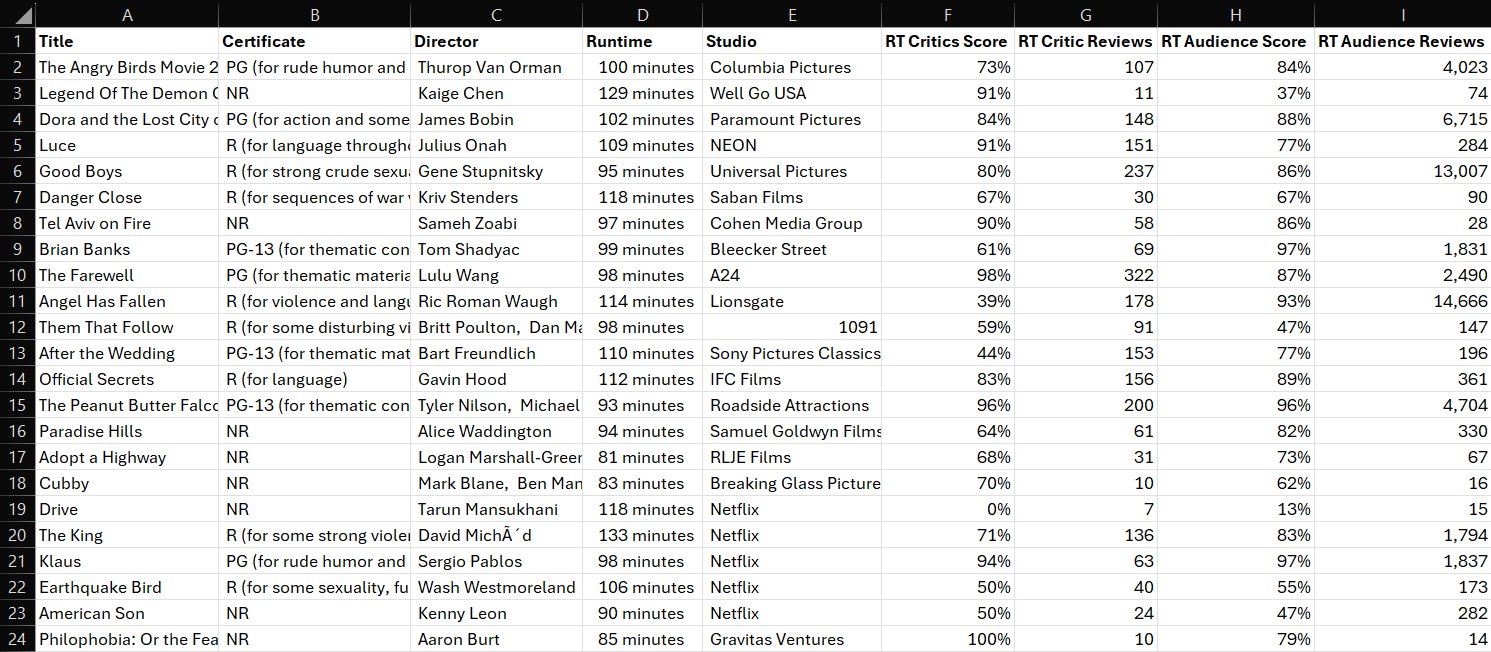
\includegraphics[width=5.2in]{figure1.png}
      \caption{The first 23 rows of the Rotten Tomatoes dataset}
      \label{Figure 1}
\end{center}
\end{figure}

\newpage

\subsubsection{Cleaning the dataset}
As seen from Figure \ref{Figure 1}, the data is not a form that is convenient for analysis. For example, the director column will have multiple names on rare occasions. Since this can throw off the analysis, we will reduce this column to only having one director. \\

\noindent Overall, this will be done for many of the columns such as Certificate, Director, RT Critics Score, and RT Audience Score. A shortened example table showing the original and desired clean dataset is shown below: \\ \\

\noindent \textbf{Original Data:}
\begin{center}
\begin{tabular}{|c|c|c|c|c|} 
\hline
\textbf{Title} & \textbf{Certificate} & \textbf{Director} & \textbf{Critics Score} & \textbf{Audience Score} \\
\hline
Light of My Life & R (for violence) & Casey Affleck & 34\% & 44\% \\
\hline
Plus One & NR & Jeff Chan,  Ari Gold & 88\% & 81\% \\
\hline
\end{tabular}
\end{center}

\qquad \\

\noindent We want to take the original data and remove any justifications for the certificate of the movie, extra directors, and percantage symbols. \\  \\

\noindent \textbf{Cleaned Data:}
\begin{center}
\begin{tabular}{|c|c|c|c|c|} 
\hline
\textbf{Title} & \textbf{Certificate} & \textbf{Director} & \textbf{Critics Score} & \textbf{Audience Score} \\
\hline
Light of My Life & R & Casey Affleck & 34 & 44 \\
\hline
Plus One & NR & Jeff Chan & 88 & 81 \\
\hline
\end{tabular}
\end{center}

\qquad \\

\noindent This cleaned data set is referenced below in Figure \ref{Figure 2}: \\

\begin{figure}[h]
\begin{center}
      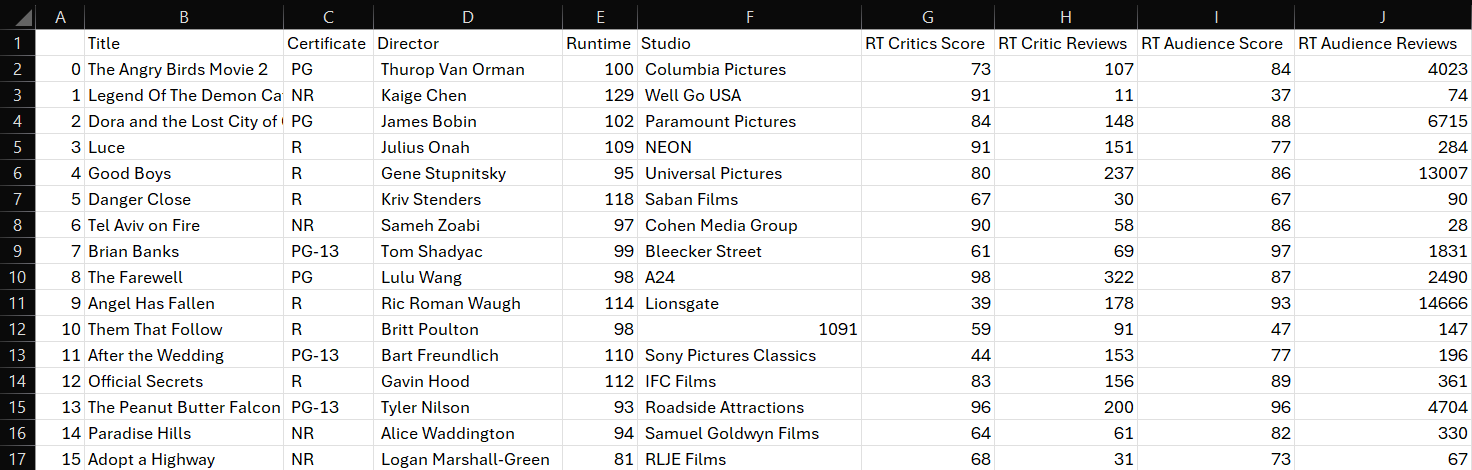
\includegraphics[width=6in]{figure2.png}
      \caption{The first 16 rows of the cleaned Rotten Tomatoes dataset}
      \label{Figure 2}
\end{center}
\end{figure}

\newpage


%%%%%%%%%%%%%%%%%%%%%%%%%%%%%%
% Rotten Tomatoes Subsection: 
%%%%%%%%%%%%%%%%%%%%%%%%%%%%%%

\subsection{iMDb}
\subsubsection{An overview of the data}

\noindent Looking at the iMDb dataset, the following information has been collected: \\
\[
\begin{array}{ll}
\text{(I) \quad Movie Poster} \qquad&\qquad \text{(VIII) \quad iMDb Metascore}  \\ \\
\text{(II) \quad Movie Title} \qquad&\qquad \text{(IX) \quad Director} \\ \\
\text{(III) \quad Year} \qquad&\qquad \text{(X) \quad Cast} \\ \\
\text{(IV) \quad Certificate} \qquad&\qquad \text{(XI) \quad Movie Description} \\ \\
\text{(V) \quad Runtime} \qquad&\qquad \text{(XII) \quad iMDb Critic Reviews} \\ \\
\text{(VI) \quad Genre} \qquad&\qquad \text{(XIII) \quad Review Title} \\ \\
\text{(VII) \quad iMDb Critics Score} \qquad&\qquad \text{(XIV) \quad Review} \\ \\

\end{array}
\]

\noindent There are 10,000 movies that have been reviewed with the above information collected. An image is attached below to help visualize this. \\

\begin{figure}[h]
\begin{center}
      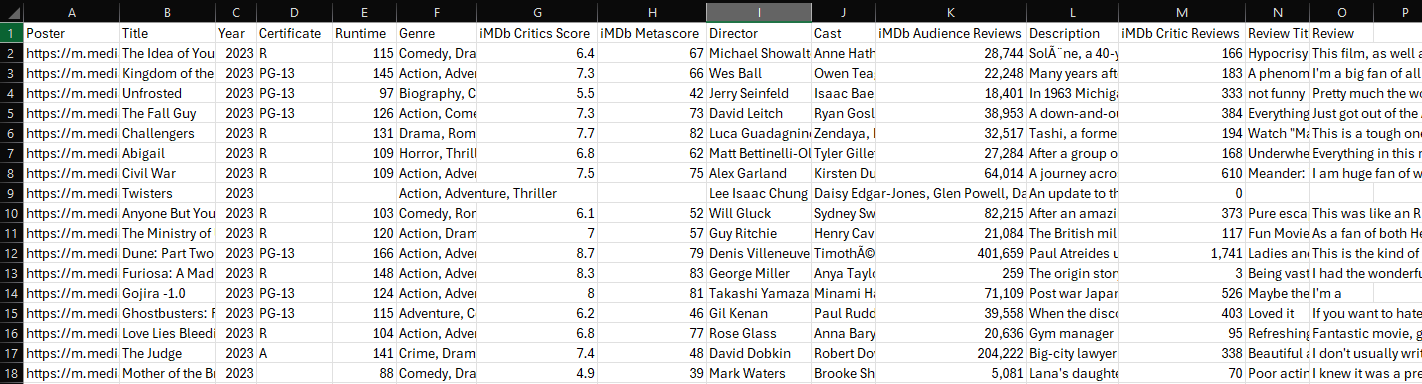
\includegraphics[width=6in]{figure3.png}
      \caption{The first 17 rows of the iMDb dataset}
      \label{Figure 3}
\end{center}
\end{figure}

\newpage

\subsubsection{Cleaning the dataset}
First, we can remove a few of the columns that don't apply to the analysis. These columns include poster, cast, description, review title, and review. \\

\noindent The genres in the iMDb dataset have the same issue as the director column in the Rotten Tomatoes dataset from Figure \ref{Figure 1}. So, the excess genres after the first will be removed. \\

\noindent The certificate column in the iMDb dataset is in terms of a rating system from India. So, a conversion is required to turn it in to the U.S. system that the Rotten Tomatoes dataset uses. In order to do this, we can refer to a table that shows equivalences between the India and U.S. certificate ratings. In python, we can use a string to string replacement. For example, this would replace a string "UA 13+" with "PG-13". This conversion code is shown below: \\

\begin{figure}[h]
\begin{center}
      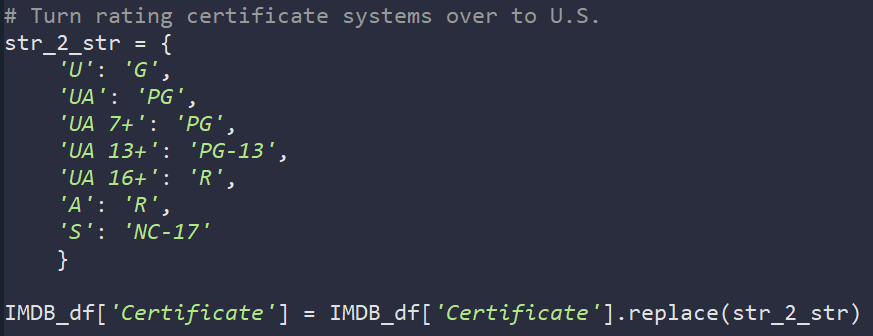
\includegraphics[width=4.5in]{figure4.png}
      \caption{The python code for India to U.S. certificate rating conversion}
      \label{Figure 4}
\end{center}
\end{figure}

\noindent This cleaned data set is referenced below in Figure \ref{Figure 5}: \\

\begin{figure}[h]
\begin{center}
      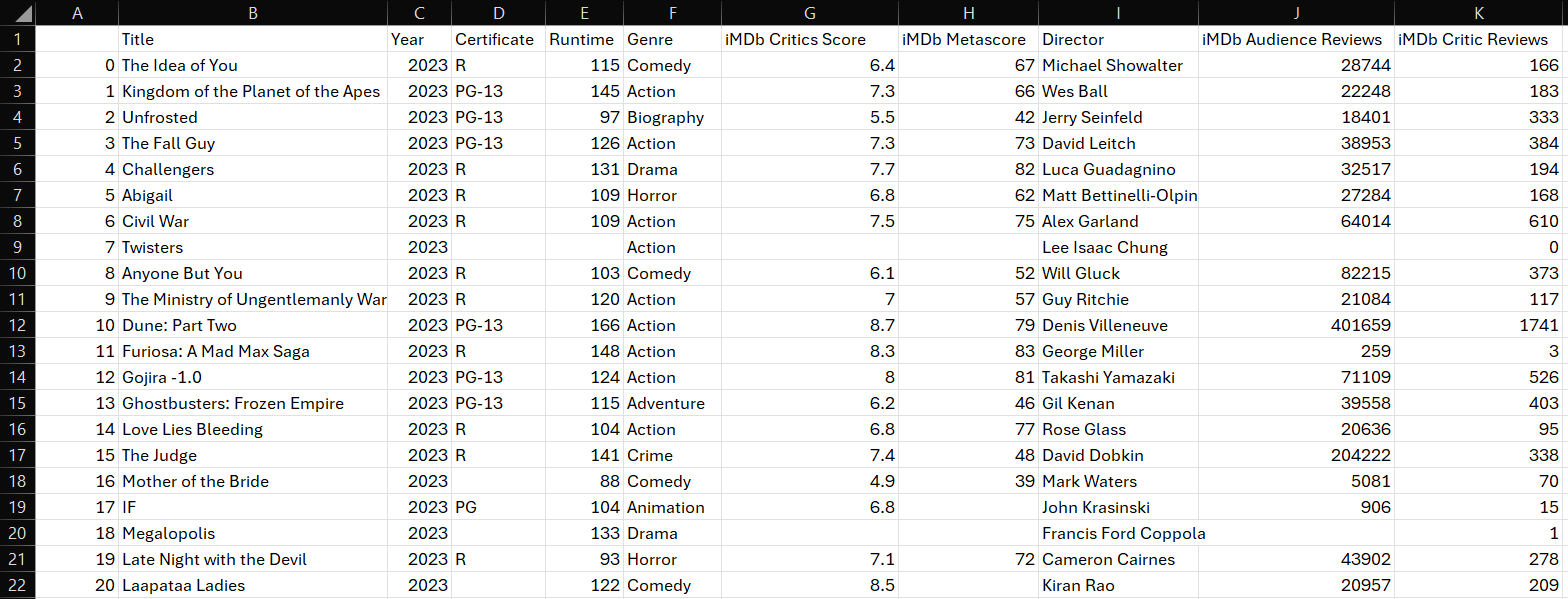
\includegraphics[width=5in]{figure5.png}
      \caption{The first 20 rows of the cleaned iMDb dataset}
      \label{Figure 5}
\end{center}
\end{figure}

\newpage

\subsection{Merging the data sets}
We can compare the two datasets more closely by looking at all of their common movies. We can achieve this by joining the two datasets based on the movie title. This will effectively be an anchor for all other data points to fill in to a new table based on that anchor. \\

\noindent However, we do need to remove some duplicate columns that are in both datasets. In python, we can achieve this by using a data-frame merge function shown below:
\begin{figure}[h]
\begin{center}
      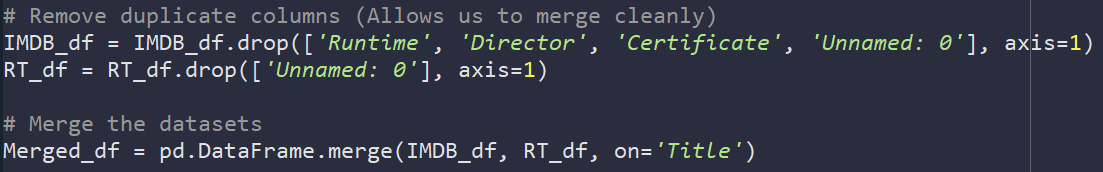
\includegraphics[width=6in]{figure6.png}
      \caption{A python function that merges dataframes based on a shared column}
      \label{Figure 6}
\end{center}
\end{figure}

\section{Results}

\subsection{Five Number Summary}
A five number summary has been produced for each of the critic's and audience's scores. \\ \\

\noindent \textbf{Five Number Summary:}
\begin{center}
\begin{tabular}{|c|c|c|c|c|c|} 
\hline
\textbf{Data} & \textbf{Minimum} & \textbf{25th Percentile} & \textbf{Median} & \textbf{75th Percentile} & \textbf{Maximum} \\
\hline
\textbf{RT Critics} & 0 & 42 & 71 & 88 & 100 \\
\hline
\textbf{RT Audience} & 5 & 43 & 61 & 76 & 100 \\
\hline
\textbf{iMDb Critics} & 13 & 58 & 65 & 72 & 97 \\
\hline
\textbf{iMDb Metascore} & 1 & 45.5 & 58 & 71 & 100 \\
\hline
\end{tabular}
\end{center}

\quad \\

\noindent Initially, it may be confusing looking at the iMDb Metascore, since it has no equivalent name in the Rotten Tomatoes dataset. On top of this, it doesn't seem to closely align with any of the other five number summaries. Another area to investigate is the mean and standard deviations of these data point. In the next subsection, we can visualize all of these values using box plots.

\newpage

\subsection{Box Plots}
In Figure \ref{Figure 7} there are four different box plots. Each vertical line represents a specific value. Going from left to right, they represent the minimum value, $\text{25}^{\text{th}}$ percentile, median, $\text{75}^{\text{th}}$ percentile, and maximum value. The mean of each box plot is also displayed by a green triangle. \\ 

\begin{figure}[h]
\begin{center}
      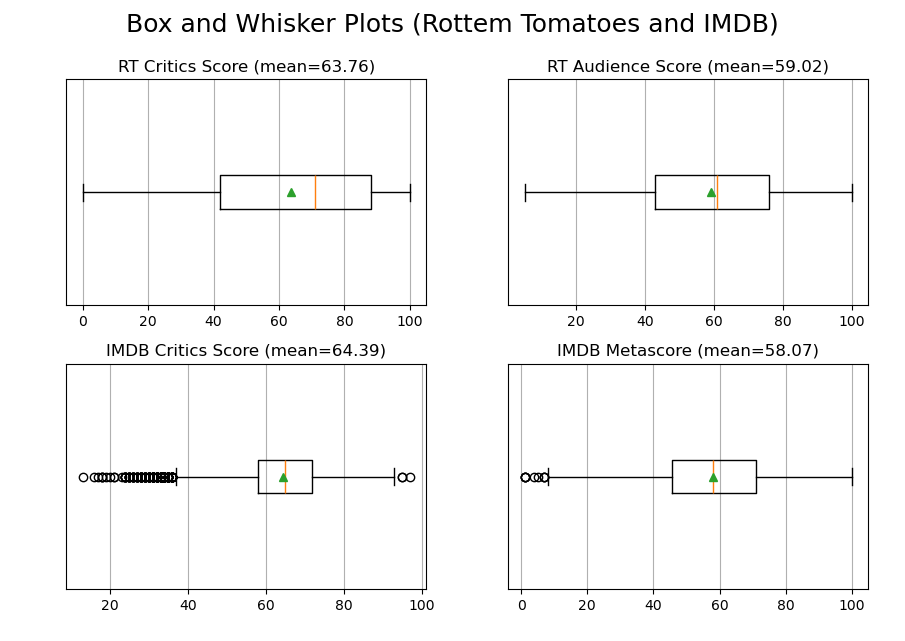
\includegraphics[width=6.25in]{figure7.png}
      \caption{Four box plots of Rotten Tomato and iMDb review scores (with means)}
      \label{Figure 7}
\end{center}
\end{figure}

\noindent Looking at the box plots, there are a few key takeaways. First, the iMDb metascore was confusing in the last subsection, however it seems like it is comparable to the Rotten Tomatoes audience score. This is due to the means having similar values. \\

\noindent Second, it seems like the Rotten Tomatoes movie scores have a larger standard deviation, as there are no detected outliers in their box plots. In other words, their ratings are more spread out across all possibilities. On the other hand, iMDb seems to have a smaller standard deviation as the boxes are smaller (25$^{\text{th}}$ and 75$^{\text{th}}$ percentiles). There are also visible outliers towards the lower end of the scores. This suggests that iMDb is more favorable to movies, but will occasionally step out of their normal trends and rate some movies on the low end (36 and below for critics).

\newpage

\subsection{iMDb Pie Chart}
A pie chart is useful for gauging relative sizes of categories. With a pie chart (Figure \ref{Figure 8}), we can visualize which movie genres have the most reviews from iMDb.

\begin{figure}[h]
\begin{center}
      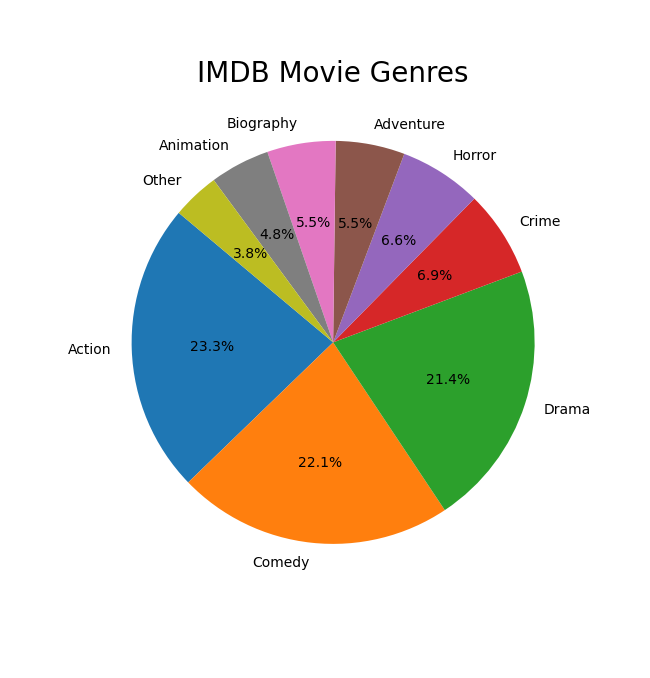
\includegraphics[width=4in]{figure8.png}
      \caption{A pie chart of iMDb movie genre counts}
      \label{Figure 8}
\end{center}
\end{figure}

\noindent It is clear to see that action, comedy, and drama movies are very common. Crime, horror, adventure, biography, and animation movies are also somewhat common. Finally, there are many movie genres in the other category are rare to see getting a review from iMDb. The following genres are rare: documentary, fantasy, thriller, mystery, sci-fi, romance, western, musical, film-noir, family, history, music, sport, and war. \\

\noindent Note: There is no chart for Rotten Tomatoes since their dataset doesn't include genres.

\newpage

\subsection{iMDb Stacked Histogram}
Another idea to investigate is how iMDb had reviewed movies with time. The stacked histogram in Figure \ref{Figure 9} shows the number of each genre for every year 2000-2025.

\begin{figure}[h]
\begin{center}
      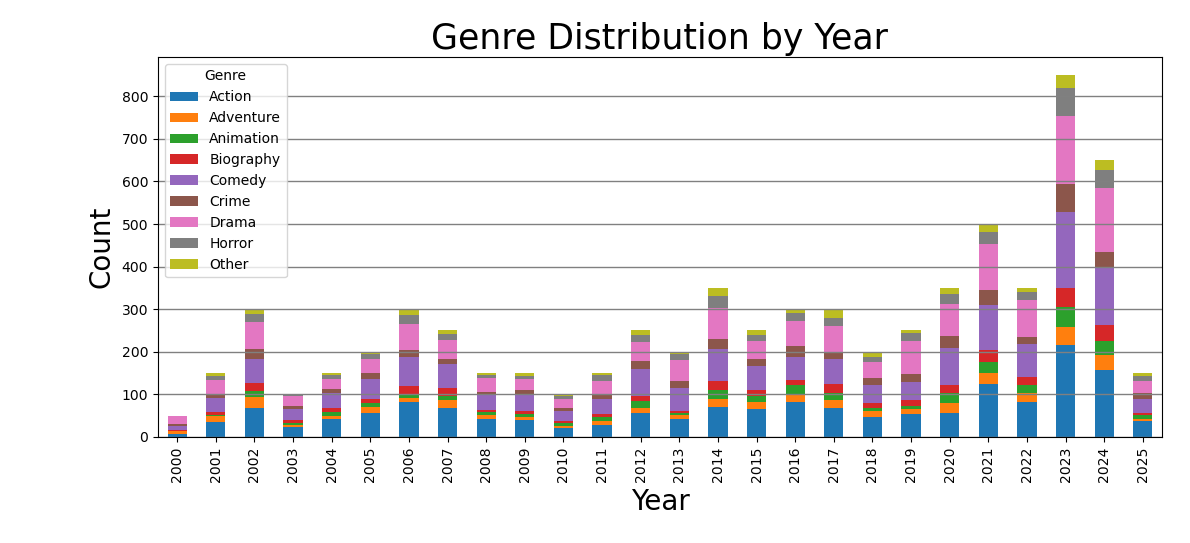
\includegraphics[width=6.5in]{figure9.png}
      \caption{A pie chart of iMDb movie genre counts}
      \label{Figure 9}
\end{center}
\end{figure}

\noindent Overall, it seems that the amount of movies has gone up overtime. What is interesting though, are the peaks in years like 2002, 2006, 2014, 2021, 2023, and 2024. For 2023, it is suspected that this is due to movie production being halted from COVID-19, and a surge of movies releasing once the pandemic slowed down. \\

\noindent It is surprising to see how the proportion of movies over the years has not changed that much. It seems like the amount of each genre is increasing/decreasing proportional to the total number of movies. \\

\noindent Something to note, though, is that its unclear if this is due to the number of movies being released, or just the proportion that iMDb is covering. Unfortunately, this is a flaw in the dataset.

\newpage

\subsection{Rotten Tomatoes Bar Chart}
In the U.S., movies are given ratings that tell the audience the intended audience of the movie. For example, G is the lowest that means everyone of all ages can watch it. On the higher end, there is rated R movies where someone under the age of 18 must be accompanied by an adult to watch the movie. And finally, there is NR which stands for not rated. \\

\noindent We can visualize how Rotten Tomatoes rates movies based on their movie certificates in Figure \ref{Figure 10} by using a bar chart.

\begin{figure}[h]
\begin{center}
      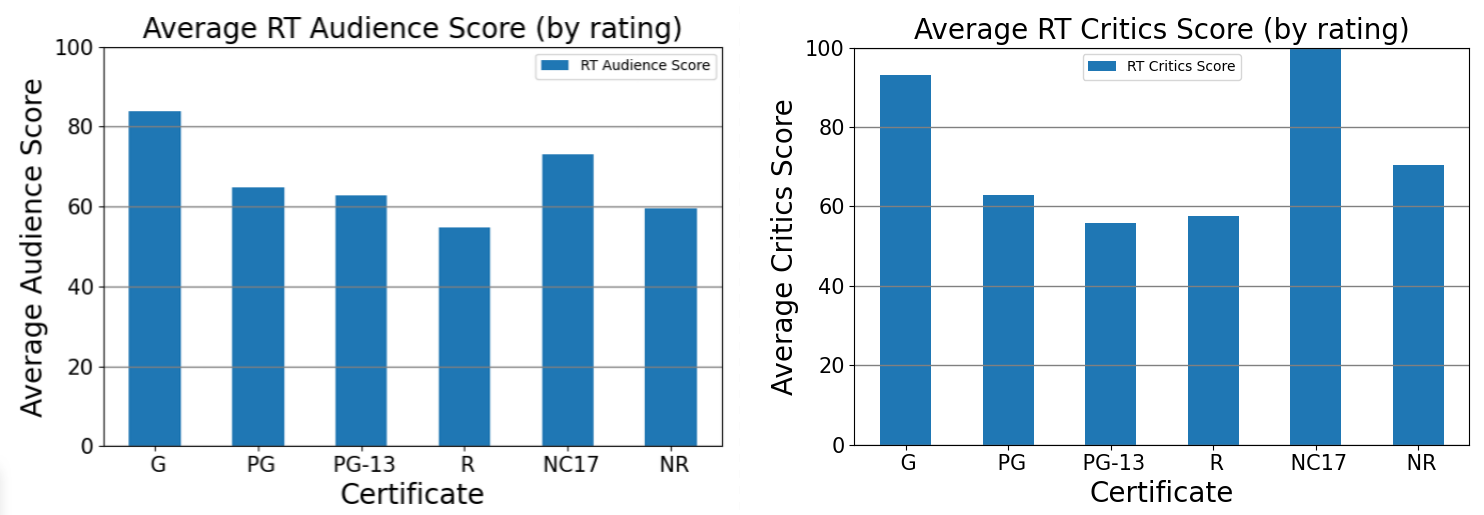
\includegraphics[width=6in]{figure10.png}
      \caption{A bar chart of Rotten Tomatoes scores by movie certificate}
      \label{Figure 10}
\end{center}
\end{figure}

\noindent There are a few things to point out about this chart. Overall, it seems like the ratings of movies decrease as the movie becomes more mature. This may seem inconsistent, though, due to the NC17 rated movies having an average RT critics score of 100. Peaking behind the curtain, though, and we can see where this discrepency is coming from: \\

\noindent \textbf{Rotten Tomatoes Critics Score by Certificate:}
\begin{center}
\begin{tabular}{|c|c|c|c|c|c|c|} 
\hline
\textbf{Certificate:} & \textbf{G} & \textbf{PG} & \textbf{PG-13} & \textbf{R} & \textbf{NC17} & \textbf{NR} \\
\hline
\textbf{Avg. RT Critics Score} & 93.17 & 62.97 & 55.76 & 57.69 & 100 & 70.32 \\
\hline
\textbf{Avg. RT Critics Score} & 84 & 64.76 & 62.81 & 54.90 & 73 & 59.54 \\
\hline
\textbf{\# of Movies} & 6 & 143 & 316 & 656 & 1 & 978 \\
\hline
\end{tabular}
\end{center}

\quad \\

\noindent It is clear to see that G and NC17 rated movies are uncredible, due to them having a sample size of 6 and 1 respectively. This is almost nothing compared to the R rated movies having a sample size os 656.

\newpage

\subsection{Merged Dataset Box Plot}
We can refine our analysis more by only focusing on movies that both companies has reviewed. This new merged data set contains 741 movies, which is credible enough to create a box plot.

\begin{figure}[h]
\begin{center}
      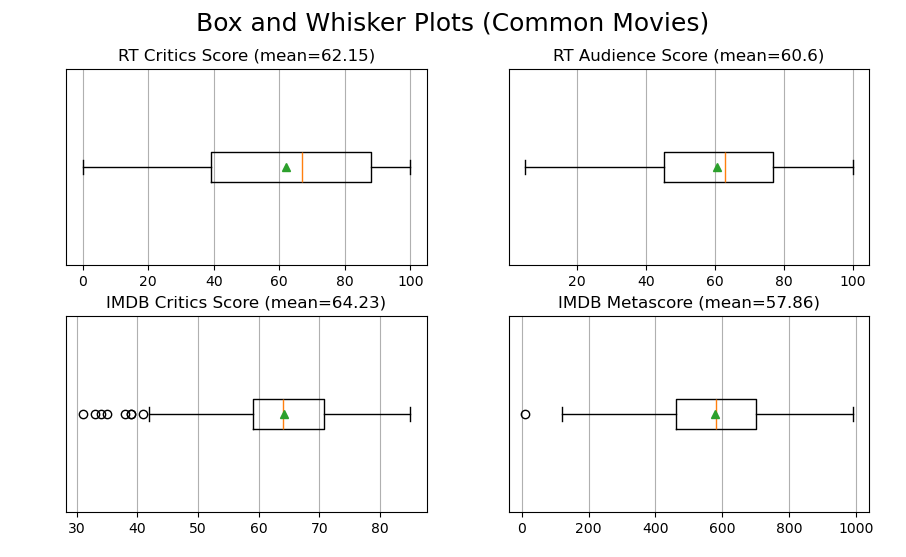
\includegraphics[width=6.5in]{figure13.png}
      \caption{A box plot of the merged data set comparing Rotten Tomatoes and iMDb}
      \label{Figure 13}
\end{center}
\end{figure}

\noindent Compared to the previous box plot in Figure \ref{Figure 7}, there is little to no change in the box plots. Due to the merging of the datasets reducing the number of movies, it looks like iMDb has fewer outliers, which is to be expected. The five number summaries and means have no practical difference.

\newpage

\section{Discussion/Conclusion}
Overall, the Rotten Tomatoes and iMDb datasets performed similarly to each other. It seems that Rotten Tomatoes and iMDb's critics are more favorable to movies while the audience is less favorable to them. It is hard to tell why that may be, but it may have to do with critics having more of an eye for artistic ability, while a general audience may not be thinking about so many factors when watching a movie. On top of this, it is very apparent that iMDb is way may consistent with critics and metascore's than Rotten Tomatoes. This is evident by looking at both box plot versions and seeing the length of each box and whisker. \\

\noindent Another interesting thing to look at is the breakdown of certificate rating and Rotten Tomatoes scores. Overall, the initial hypothesis was that critics and audience scores rating would be down as movies got more mature, more-so for the critics score. But, this was not seen at all. It seems that both the critics and audience liked NR rated movies more than anything other than G rated movies. The only exception to this are the NC17 movies, but those can be ignored since they only have a sample size of one.

\section{Resources}
\quad \\
\begin{enumerate}
    \item \href{https://brooksemerick.com/s/RottenTomatoes.csv}{Rotten Tomatoes Dataset} \\
    \item \href{https://brooksemerick.com/s/iMDb.csv}{iMDb Dataset}
\end{enumerate}




\end{document}